% ---------------------------------------------------------------------------
% Quelle der Abbildung:
%   Skript:  thesis/figures/scripts/kegelstrahl_geometrie.py (analytisch, kein Trainingslauf)
%   Aufruf:  /tmp/holo311/bin/python thesis/figures/scripts/kegelstrahl_geometrie.py
%   Basis:   Commit 1abccf9 (Branch cursor/thesis-grundlagen-6175), 2026-10-01
%   Dateien: kegelstrahl_geometrie.pdf
% Einbinden im Kapitel: % ---------------------------------------------------------------------------
% Quelle der Abbildung:
%   Skript:  thesis/figures/scripts/kegelstrahl_geometrie.py (analytisch, kein Trainingslauf)
%   Aufruf:  /tmp/holo311/bin/python thesis/figures/scripts/kegelstrahl_geometrie.py
%   Basis:   Commit 1abccf9 (Branch cursor/thesis-grundlagen-6175), 2026-10-01
%   Dateien: kegelstrahl_geometrie.pdf
% Einbinden im Kapitel: % ---------------------------------------------------------------------------
% Quelle der Abbildung:
%   Skript:  thesis/figures/scripts/kegelstrahl_geometrie.py (analytisch, kein Trainingslauf)
%   Aufruf:  /tmp/holo311/bin/python thesis/figures/scripts/kegelstrahl_geometrie.py
%   Basis:   Commit 1abccf9 (Branch cursor/thesis-grundlagen-6175), 2026-10-01
%   Dateien: kegelstrahl_geometrie.pdf
% Einbinden im Kapitel: % ---------------------------------------------------------------------------
% Quelle der Abbildung:
%   Skript:  thesis/figures/scripts/kegelstrahl_geometrie.py (analytisch, kein Trainingslauf)
%   Aufruf:  /tmp/holo311/bin/python thesis/figures/scripts/kegelstrahl_geometrie.py
%   Basis:   Commit 1abccf9 (Branch cursor/thesis-grundlagen-6175), 2026-10-01
%   Dateien: kegelstrahl_geometrie.pdf
% Einbinden im Kapitel: \input{figures/grundlagen/kegelstrahl_geometrie}
% ---------------------------------------------------------------------------
\begin{figure}[tbp]
  \centering
  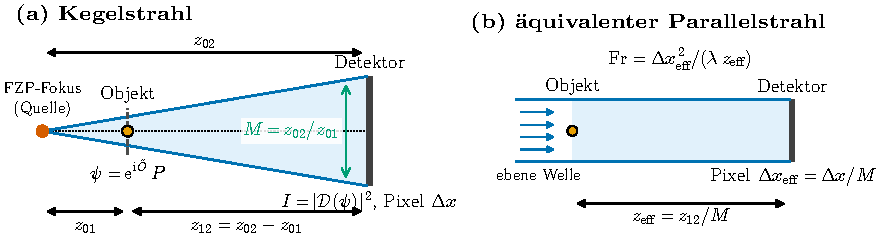
\includegraphics[width=\textwidth]{figures/grundlagen/kegelstrahl_geometrie}
  \caption[Kegelstrahlgeometrie der Nahfeldholographie und äquivalenter Parallelstrahl]{%
    Kegelstrahlgeometrie der \acs{nfh} (schematisch, nicht maßstäblich).
    (a)~Der Fokus der Fresnel-Zonenplatte wirkt als virtuelle Punktquelle; das
    Objekt im Abstand $\zOne$ wird mit $\magn = \zTwo/\zOne$ vergrößert auf den
    Detektor im Abstand $\zTwo$ abgebildet. (b)~Nach dem
    Fresnel-Skalierungstheorem ist die Aufnahme äquivalent zu einer
    Parallelstrahl-Propagation über $\zEff = (\zTwo-\zOne)/\magn$ bei effektiver
    Pixelgröße $\dx/\magn$; beides zusammen definiert die Fresnel-Zahl
    (\cref{eq:grundlagen:fresnelzahl}).}
  \label{fig:grundlagen:kegelstrahl}
\end{figure}

% ---------------------------------------------------------------------------
\begin{figure}[tbp]
  \centering
  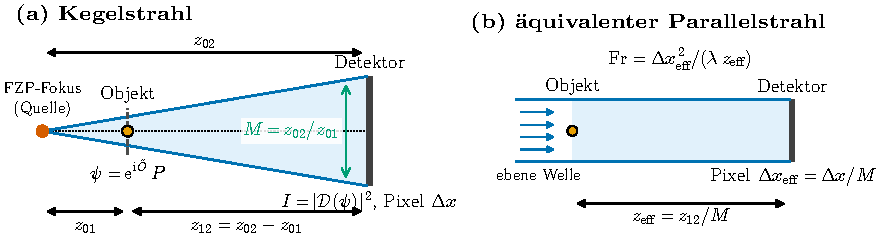
\includegraphics[width=\textwidth]{figures/grundlagen/kegelstrahl_geometrie}
  \caption[Kegelstrahlgeometrie der Nahfeldholographie und äquivalenter Parallelstrahl]{%
    Kegelstrahlgeometrie der \acs{nfh} (schematisch, nicht maßstäblich).
    (a)~Der Fokus der Fresnel-Zonenplatte wirkt als virtuelle Punktquelle; das
    Objekt im Abstand $\zOne$ wird mit $\magn = \zTwo/\zOne$ vergrößert auf den
    Detektor im Abstand $\zTwo$ abgebildet. (b)~Nach dem
    Fresnel-Skalierungstheorem ist die Aufnahme äquivalent zu einer
    Parallelstrahl-Propagation über $\zEff = (\zTwo-\zOne)/\magn$ bei effektiver
    Pixelgröße $\dx/\magn$; beides zusammen definiert die Fresnel-Zahl
    (\cref{eq:grundlagen:fresnelzahl}).}
  \label{fig:grundlagen:kegelstrahl}
\end{figure}

% ---------------------------------------------------------------------------
\begin{figure}[tbp]
  \centering
  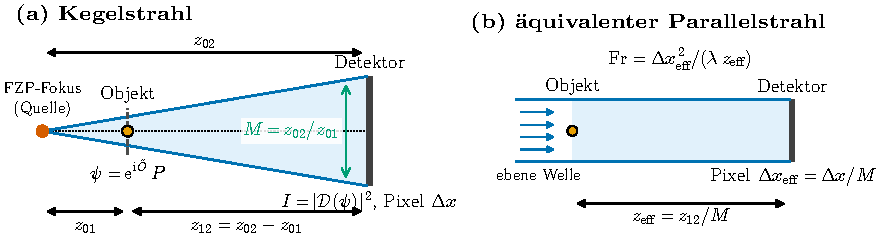
\includegraphics[width=\textwidth]{figures/grundlagen/kegelstrahl_geometrie}
  \caption[Kegelstrahlgeometrie der Nahfeldholographie und äquivalenter Parallelstrahl]{%
    Kegelstrahlgeometrie der \acs{nfh} (schematisch, nicht maßstäblich).
    (a)~Der Fokus der Fresnel-Zonenplatte wirkt als virtuelle Punktquelle; das
    Objekt im Abstand $\zOne$ wird mit $\magn = \zTwo/\zOne$ vergrößert auf den
    Detektor im Abstand $\zTwo$ abgebildet. (b)~Nach dem
    Fresnel-Skalierungstheorem ist die Aufnahme äquivalent zu einer
    Parallelstrahl-Propagation über $\zEff = (\zTwo-\zOne)/\magn$ bei effektiver
    Pixelgröße $\dx/\magn$; beides zusammen definiert die Fresnel-Zahl
    (\cref{eq:grundlagen:fresnelzahl}).}
  \label{fig:grundlagen:kegelstrahl}
\end{figure}

% ---------------------------------------------------------------------------
\begin{figure}[tbp]
  \centering
  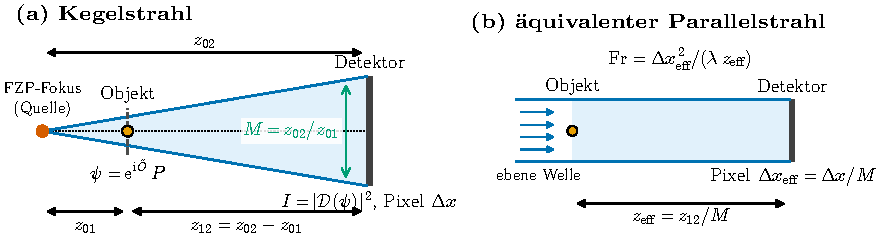
\includegraphics[width=\textwidth]{figures/grundlagen/kegelstrahl_geometrie}
  \caption[Kegelstrahlgeometrie der Nahfeldholographie und äquivalenter Parallelstrahl]{%
    Kegelstrahlgeometrie der \acs{nfh} (schematisch, nicht maßstäblich).
    (a)~Der Fokus der Fresnel-Zonenplatte wirkt als virtuelle Punktquelle; das
    Objekt im Abstand $\zOne$ wird mit $\magn = \zTwo/\zOne$ vergrößert auf den
    Detektor im Abstand $\zTwo$ abgebildet. (b)~Nach dem
    Fresnel-Skalierungstheorem ist die Aufnahme äquivalent zu einer
    Parallelstrahl-Propagation über $\zEff = (\zTwo-\zOne)/\magn$ bei effektiver
    Pixelgröße $\dx/\magn$; beides zusammen definiert die Fresnel-Zahl
    (\cref{eq:grundlagen:fresnelzahl}).}
  \label{fig:grundlagen:kegelstrahl}
\end{figure}
